\documentclass[a4paper, 7pt, landscape]{scrartcl}
\usepackage[german]{babel}
\usepackage[utf8]{inputenc}
\usepackage{multicol}
\usepackage{geometry}
\usepackage{graphicx}
\usepackage{wrapfig}
\usepackage{enumitem}
\usepackage{fancyhdr}
\usepackage{index}
\usepackage{sectsty}
\usepackage{mwe}
\usepackage{comment}
\usepackage{lipsum}
\usepackage{titlesec}
\usepackage[dvipsnames]{xcolor}
\usepackage{amsmath}
\usepackage{amssymb}
\usepackage{listings}


%Define Math Commands:
\newcommand*{\field}[1]{\mathbb{#1}}%
\newcommand{\Mod}[1]{\ (\mathrm{mod}\ #1)}

%Image Folder:
\graphicspath{{../img/}}

%format
\geometry{top=0.4cm,left=0.5cm,right=0.5cm,bottom=0.4cm}
\setlist{topsep=0pt, leftmargin=5mm, nolistsep}

% Code Snippets

\definecolor{javared}{rgb}{0.6,0,0} % for strings

\lstset{
language=C,
basicstyle=\fontsize{7}{7} \ttfamily,
keywordstyle=\bfseries\color{RoyalBlue},
stringstyle=\color{javared},
commentstyle=\color{MidnightBlue},
morecomment=[s][\color{MidnightBlue}]{/**}{*/},
tabsize=2,
showspaces=false,
showstringspaces=false,
texcl = true,
rulecolor = \color{black},
breaklines = true,
aboveskip = 0em,
belowskip = 0em
}




% Define Section Format
\titleformat{name=\section}[block]
{\sffamily\normalsize}
{}
{0pt}
{\colorsection}
\titlespacing*{\section}{0pt}{0pt}{0pt}

\newcommand{\colorsection}[1]{%
\colorbox{MidnightBlue!40}{\parbox{0.98\linewidth}{\color{black}\thesection\ #1}}}


% Define Subsection Format
\titleformat{name=\subsection}[block]
{\sffamily\small}
{}
{0pt}
{\colorsubsection}
\titlespacing*{\subsection}{0pt}{0pt}{0pt}

\newcommand{\colorsubsection}[1]{%
\colorbox{YellowGreen!50}{\parbox{0.98\linewidth}{\color{black}\thesubsection\ #1}}}

% Define SubSubsection Format
\titleformat{name=\subsubsection}[block]
{\sffamily\small}
{}
{0pt}
{\colorsubsubsection}
\titlespacing*{\subsubsection}{0pt}{0pt}{0pt}

\newcommand{\colorsubsubsection}[1]{%
\colorbox{Goldenrod!50}{\parbox{0.98\linewidth}{\color{black}\thesubsubsection\ #1}}}


% -----------------------------------------------------------------------
\begin{document}
    %	\pagecolor{p}
    %	\color{t}
    \setlength{\columnseprule}{0.4pt}
    \footnotesize
    \begin{multicols*}{3}

        %! Author = phili
%! Date = 25/06/2021

\section{Secure Software Principles}
\textbf{Three pillars}
\begin{itemize}
    \item Risk Management
    \item Touchpoints
    \item Knowledge
\end{itemize}

\subsection{80\% / 20\% Problem Reduction}
\begin{enumerate}
    \item Secure the weakest link
    \item Practice defence in depth
    \item Fail securely
    \item Follow the principle of least privilege
    \item Compartmentalize
    \item Keep it simple
    \item Promote privacy
    \item Remember that hiding secrets is hard
    \item Be reluctant to trust (Off-the-shelf software)
    \item Use your community resources (crypto algorithms)
\end{enumerate}


        %! Author = phili
%! Date = 25/06/2021

\section{Secure Software Lifecycle}
\textbf{SW Engineering processes:} Waterfall, Spiral, Prototyping, XP, Adaptive Programming, ...\\
None of these really support security.\\

\subsection{Software Engineering \& Security}
\begin{itemize}
    \item Often ad hoc or not covered at all
    \item Issues:
    \begin{itemize}
        \item Non systematic approach
        \item Bad early decisions
        \item Hard to manage and modify
    \end{itemize}
\end{itemize}
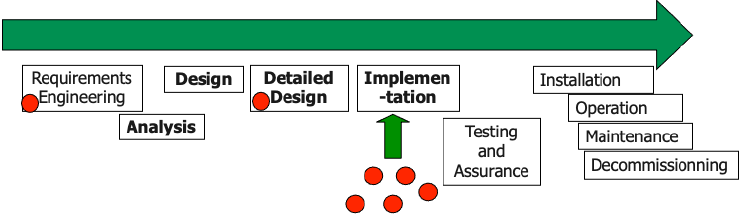
\includegraphics[width=\linewidth]{../img/sw_engineering_security.png}

\subsection{Requirements / Analysis}
\begin{itemize}
    \item Identify security requirements
    \item Quantify the security risks
    \item Know the entire problem domain of the system
\end{itemize}

\subsubsection{Identify Security Requirements}
\begin{enumerate}
    \item Identify stakeholders
    \item Identify assets from different stakeholders (sensitive info / resources)
    \item Identify requirements on these assets
\end{enumerate}
\textbf{Result:} high-level security policy\\
\textbf{STRIDE:} Systematic approach for threat identification.
\begin{itemize}
    \item \textbf{S}poofing
    \item \textbf{T}ampering
    \item \textbf{R}epudiation
    \item \textbf{I}nformation disclosure
    \item \textbf{D}enial of service
    \item \textbf{E}levation of privilege
\end{itemize}

\subsubsection{Quantify Security Risks}
\begin{itemize}
    \item Estimate and quantify the risk of the previously identified threats
    \begin{enumerate}
        \item Importance or severity (critical vs. non-critical)
        \item Cost
        \item DREAD (Damage potential, Reproduceability, Exploitability, Affected users, Discoverability)
    \end{enumerate}
    \item Order the requirements and identify the relevant subset: Risk mitigation strategy
\end{itemize}
\textbf{Result:} high-level security policy revisited

\subsubsection{Example}
\textbf{General formulated:}\\
\textit{The software must validate all user input to ensure it does not exceed the size specified fot that type of input.}\\
\textit{The system must encrypt sensitive data transmitted over the Internet between the server and the browser.}\\
\textbf{Non-functional requirements:}\\
\begin{enumerate}
    \item \textbf{Security Property Requirement}: specifies the characteristics that software must exhibit.
    \item \textbf{Constraint or Negative Requirements} limit what software functionality can be allowed to behave.
    \item \textbf{Security Assurance Requirements} are rules or best practices by which the software security functions will be built, deployed and operated.
\end{enumerate}

\subsection{Detailed Design}
\textbf{Main goals:}\\
\begin{enumerate}
    \item Identify security technologies that meet relevant security requirements
    \item Bind these technologies to the application
\end{enumerate}

\subsubsection{Identify security technologies}
\begin{itemize}
    \item Select requirements that should be addressed at this level
    \item Identify security technologies that address requirements
\end{itemize}
\textbf{STRIDE Countermeasures:}
\textbf{Tampering}
\begin{itemize}
    \item Use data hashing and signing
    \item Digital signatures
    \item Strong authorization
    \item Tamper-resistant protocols across communication links
    \item Secure communication links with protocols that provide message integrity
\end{itemize}
\textbf{Information Disclosure}
\begin{itemize}
    \item Strong authorization
    \item Strong encryption
    \item Secure communication links with protocols that provide message confidentiality
    \item Do not store secrets in plaintext
\end{itemize}
...

\subsubsection{Bind Technologies to Application}
\begin{itemize}
    \item For coarse-grained or simple requirements
    \begin{itemize}
        \item Countermeasure can be realized in the operating system/middleware (SSL)
    \end{itemize}
    \item For fine-grained and complex requirements
    \begin{itemize}
        \item Implement as part of the application (hard to get right)
    \end{itemize}
\end{itemize}

\subsection{Other phases}
\begin{itemize}
    \item Avoiding implementation vulnerabilities
    \item Security testing
    \item Automated patching
\end{itemize}

\subsection{Case study: Web Applications}
\subsubsection{High level Architecture}
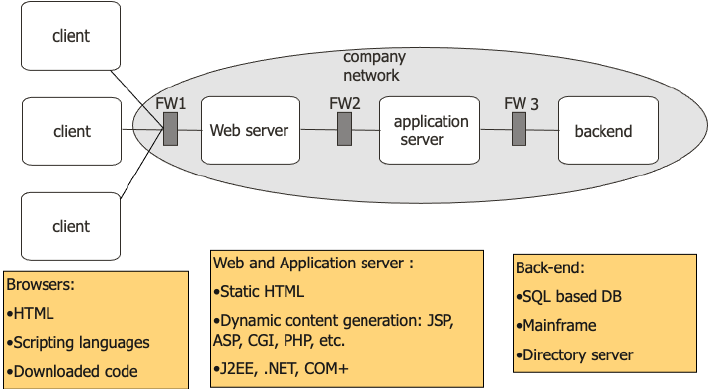
\includegraphics[width=\linewidth]{../img/web_application.png}
\subsubsection{Owners and Assets}
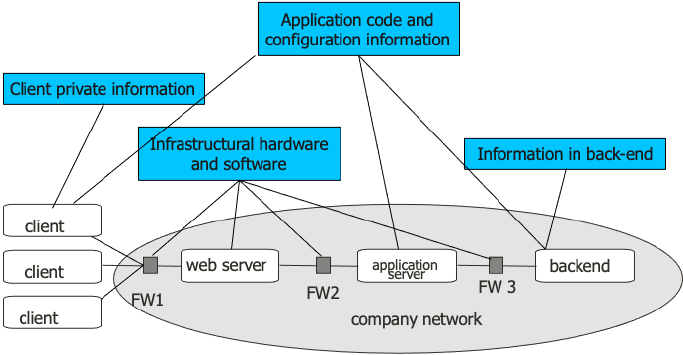
\includegraphics[width=\linewidth]{../img/web_application_owners_assets.png}
\subsubsection{Threat Agents and Threats}
\textbf{Any hacker on the internet:}
\begin{itemize}
    \item Spoof client or server
    \item Eavesdrop on connections / modify data in transit
    \item Bring down infrastructure components
    \item Gain unauthorized access to application or data
\end{itemize}
\textbf{Authorized user of the application: (additionally)}
\begin{itemize}
    \item Repudiate transactions
    \item Elevate privilege
\end{itemize}
\textbf{Malicious server:}
\begin{itemize}
    \item Steal private client information
    \item Spread spyware/viruses
\end{itemize}

\subsubsection{Infrastructural countermeasures}
\textbf{Authentication:}
\begin{itemize}
    \item Network level: IPSEC
    \item Transport level: HTTP authentication mechanisms
    \item OS level: Windows authentication
    \item Single sing-on systems based on federation or windows active directory (Kerberos)
    \item Web authentication products: IAM products
\end{itemize}
\textbf{Data protection:}
\begin{itemize}
    \item IPSEC (Network)
    \item Kerberos (OS)
    \item TLS (Transport)
\end{itemize}
\textbf{Access control:}
\begin{itemize}
    \item Firewall
    \item In the webserver (URL)
    \item RBAC in the web container or application server
    \item File system based access control
    \item Access control products
\end{itemize}
\textbf{Sandboxing:}
\begin{itemize}
    \item At the OS level: low-privileged accounts
    \item Language level: Java security architectures
\end{itemize}
\textbf{Others:}
\begin{itemize}
    \item Filtering
    \item Throttling
    \item Shielding
    \item ...
\end{itemize}

\subsubsection{Typical vulnerabilities}
\textbf{Bugs in functional parts}
\begin{itemize}
    \item Input validation
    \item Race conditions
    \item Bad error handling
\end{itemize}
\textbf{Broken countermeasures}
\begin{itemize}
    \item Access control
    \item Authentication
    \item Crypto
\end{itemize}

\subsubsection{Available Countermeasures at coding level}
\begin{itemize}
    \item Security technologies
    \item Quality improvements
    \begin{itemize}
        \item Choice of programming language
        \item Coding guidelines
        \item Source code scanners
        \item Security testing and audit
        \item Code review
    \end{itemize}
\end{itemize}

\subsection{Daily Sins}
\begin{enumerate}
    \item Buffer Overruns
    \item Format String problems
    \item Integer Overflows
    \item SQL Injection
    \item Command Injection
    \item Failing to Handle Errors
    \item XSS
    \item Failing to protect Network traffic
    \item Use of magic URLs and Hidden Forms
    \item Improper use of SSL and TLS
    \item Use of Weak Password-Based systems
    \item Failing to store and protect data securely
    \item Information leakage
    \item Improper file access
    \item Trusting Network Name Resolution
    \item Race Conditions
    \item Unauthenticated Key Exchange
    \item Cryptographically strong random numbers
    \item Poor usability
\end{enumerate}
        %! Author = phili
%! Date = 25/06/2021

\section{Threat Modeling}
\subsection{Securing DevOps}
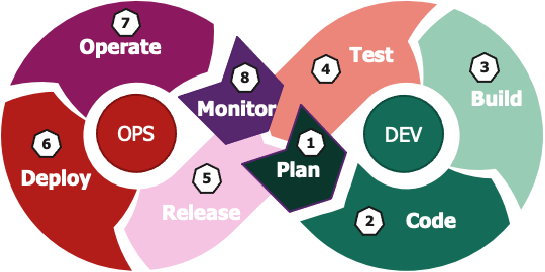
\includegraphics[width=0.5\linewidth]{../img/devops_infinity.png}
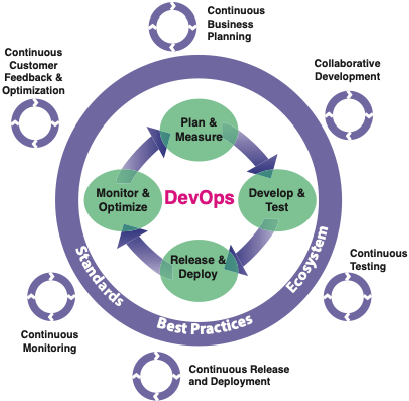
\includegraphics[width=0.5\linewidth]{../img/devops_reference_architecture.png}

\subsection{Four Major Activities}
\begin{itemize}
    \item Plan and measure
    \item Develop and test
    \item Release and deploy
    \item Monitor and optimize
\end{itemize}

\subsection{Continous Secutity}
\begin{itemize}
    \item Prepare the organisation
    \item Protect the software
    \item Produce well secured software
    \item Respond to vulnerabilities
\end{itemize}

\subsection{Security in the Phases}
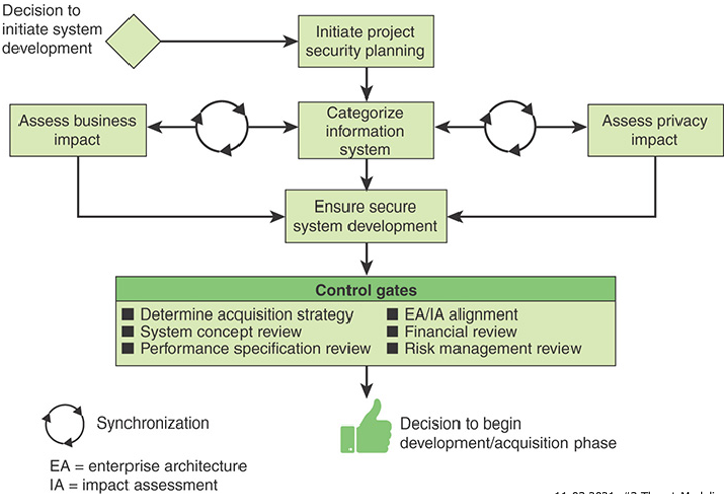
\includegraphics[width=\linewidth]{../img/security_in_phases.png}
\textbf{Major Security Activities:} A number of
security-related activities are needed to assure
that security is incorporated effectively in that
design phase\\
\textbf{Expected Outputs:} A key to success is to
define specific deliverables for each activity\\
\textbf{Synchronization:} A feedback loop between
tasks provides opportunities to ensure that the
SDLC is implemented as a flexible approach
that allows for appropriate and consistent
communication and the adaptation of tasks and
deliverables as the system is developed\\
\textbf{Control gates:} Decision points at the end of
each phase when the system is evaluated and
management determines whether the project
should continue as is, change direction, or be
discontinued\\

\subsubsection{Initiate project security planning}
\begin{itemize}
    \item Identify key security roles
    \item Identify the standards and regulations for the system
    \item Develop an overall plan for security milestones
    \item Get Stakeholders to have a common understanding (security implications, considerations, requirements)
    \item Enable developers to design security features
    \item \textbf{Output:} Supporting documents of all decisions
\end{itemize}

\subsubsection{Categorize information system}
\begin{itemize}
    \item Identify information that will be transmitted, processed or stored
    \item Define applicable levels of information categorization (based on impact analysis)
    \item \textbf{Result:} Catalog of information types
    \item \textbf{Outputs:} Definitions of categories, level of effort estimate
\end{itemize}

\subsubsection{Ensuring secure system development}
\begin{itemize}
    \item Develop a set of principles of security expectations
    \begin{itemize}
        \item Secure concept of operations
        \item Standards and processes
        \item Security training for development team
        \item Quality management
        \item Secure environment
        \item Secure code practices and repositories
    \end{itemize}
    \item \textbf{Output:} Plans for development security training / quality assurance
\end{itemize}

\subsubsection{Control Gates}
\begin{itemize}
    \item Determine acquisition strategy
    \item System concept review
    \item Performance specification review
    \item EA/IA alignment
    \item Financial review
    \item Risk management review
\end{itemize}

\subsection{Develop \& Test}
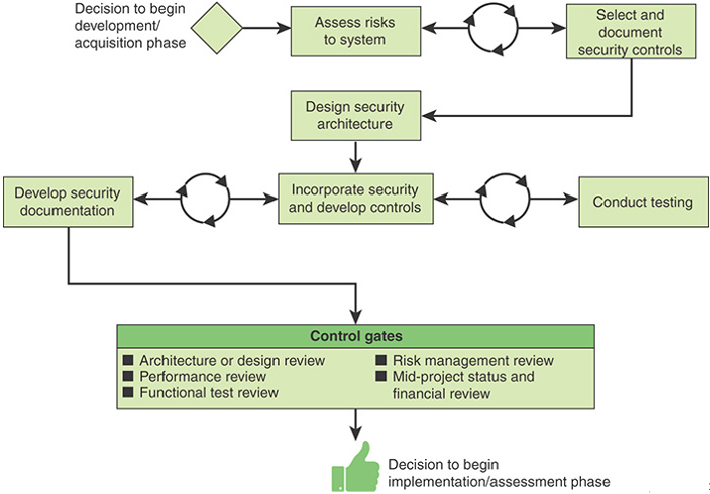
\includegraphics[width=\linewidth]{../img/develop_and_test.png}

\subsubsection{Designing the security architecture}
\begin{itemize}
    \item Produce a detailed architecture
    \item Incorporate security features and controls into the system design
    \item \textbf{Outputs:} 
    \begin{itemize}
        \item Schematic of security integration
        \item List of shared services
        \item Identification of common controls used by the system
    \end{itemize}
\end{itemize}

\subsubsection{Control Gates}
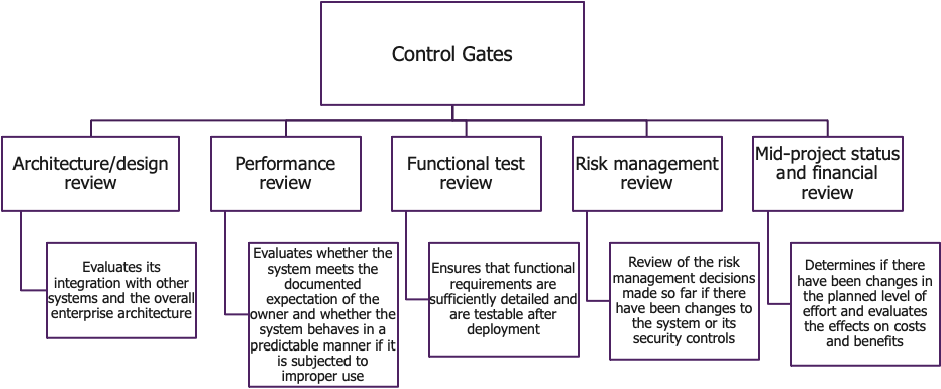
\includegraphics[width=\linewidth]{../img/control_gates.png}

\subsubsection{Begin Implementation / Assessment phase}
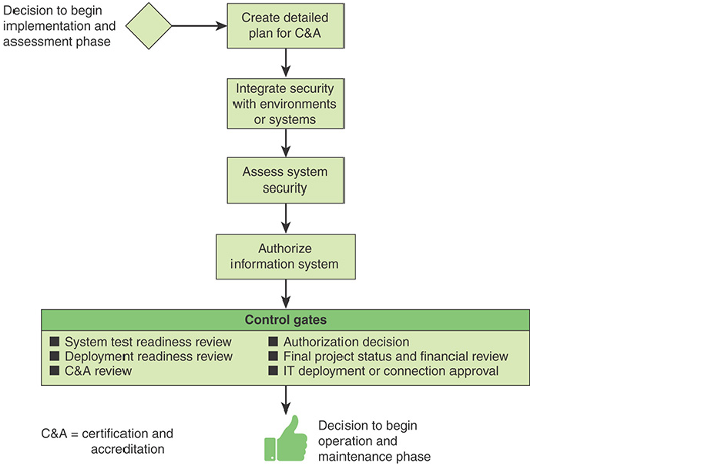
\includegraphics[width=\linewidth]{../img/develop_and_test2.png}

\subsubsection{Control Gates}
\begin{itemize}
    \item System test readiness review
    \item Deployment readiness review
    \item Certification and accreditation review
    \item Authorization decision
    \item Final project status and financial review
    \item IT deployment or connection approval
\end{itemize}

\subsubsection{Begin Operations and Maintenance phase}
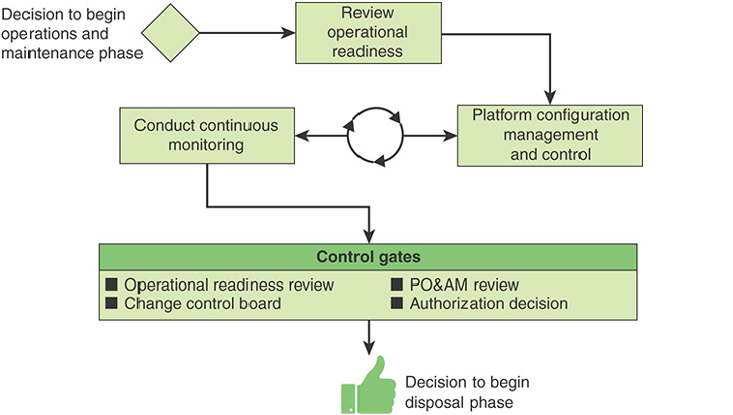
\includegraphics[width=\linewidth]{../img/develop_and_test3.png}

\subsubsection{Initiate disposal phase}
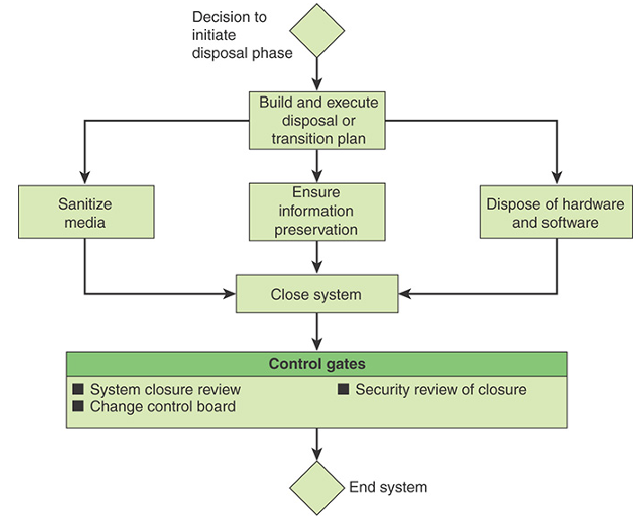
\includegraphics[width=\linewidth]{../img/develop_and_test4.png}

\subsection{Continous Security}
\begin{enumerate}
    \item Test driven Security
    \item Monitor and respond to attacks
    \item Assess risks and mature security
\end{enumerate}

\subsection{Risk Management}
\subsubsection{Activities}
\textbf{Summary:}\\
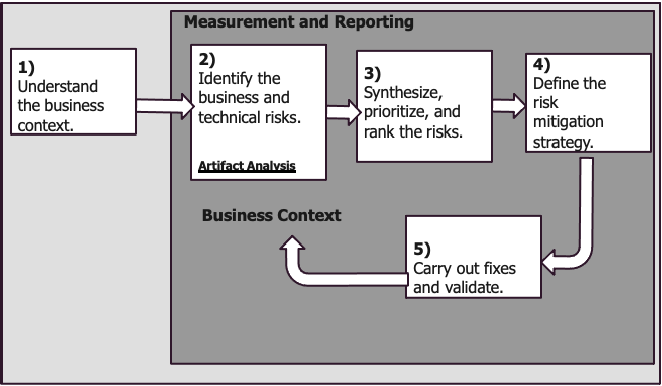
\includegraphics[width=\linewidth]{../img/risk_management_activities.png}
\begin{enumerate}
    \item Understand the business context
    \begin{itemize}
        \item Extract and describe business goals
        \item Set prios
        \item Understanding what risks to consider
        \item Gathering the artifacts
        \item Conducting project research to the scope
    \end{itemize}
    \item Identifying the business and technical risks (priorize / rank)
    \begin{itemize}
        \item Business risks impact business goals
        \item Map technical risks to business goals
        \item Develop a set of risk questionnaires
        \item Interview the target project team
        \item Analyse the research interview data
        \item Evaluate software artifacts
    \end{itemize}
    \item Synthesize, prioritize and rank the risks
    \begin{itemize}
        \item Prio the risks based on business goals
        \item Apply risk metrics
        \item Number of risks emerging over time
        \item What shall be done first?
        \item What is the best allocation of resources?
    \end{itemize}
    \item Define the risk mitigation strategy
    \begin{itemize}
        \item Take into account: Cost, Implementation time, Likelihood of success, Competence and impact
        \item Identify the validation techniques
        \item Metrics are financial in nature
    \end{itemize}
    \item Carry out fixes and validate their correctness
    \begin{itemize}
        \item Implement the mitigation strategy
        \item Rectify artifacts
    \end{itemize}
\end{enumerate}

\subsubsection{Summary}
\begin{itemize}
    \item Relies on continuous and consistent identification of risks.
    \item The five fundamentals should be applied repeatedly
    \item Use project management tools to track risk information
\end{itemize}

\subsection{Attack Trees}
\begin{itemize}
    \item Tree-structured graph
    \item Showing how a system can be attacked
\end{itemize}
\textbf{Construction:}
\begin{enumerate}
    \item Identify goals (1 Tree per goal)
    \item Identify attacks against goals
    \item Existing sub-trees can be plugged in
\end{enumerate}
\textbf{Usage:}
\begin{itemize}
    \item Propagate up the tree
    \item You can specify values that represent other different meanings (Equipment / Cost)
    \item Combine Node Values
\end{itemize}

\subsubsection{Example}
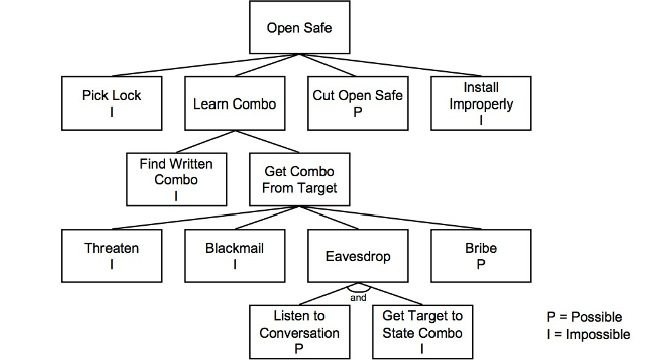
\includegraphics[width=\linewidth]{../img/attack_tree_example.png}
\textbf{Countermeasures:}\\ 
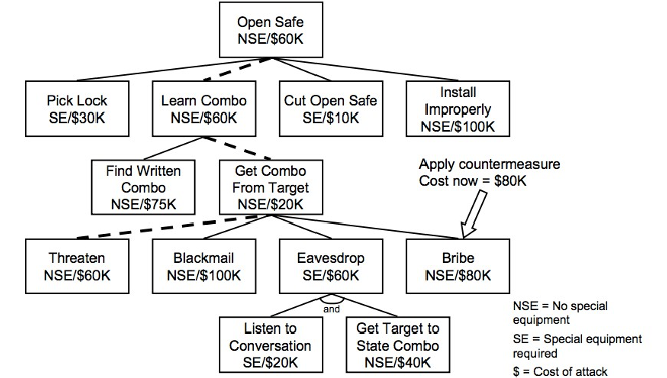
\includegraphics[width=\linewidth]{../img/attack_tree_example2.png}

        %! Author = phili
%! Date = 28/06/2021

\section{Threats \& Attacks}
\subsection{Threat Risk Modeling}
\begin{enumerate}
    \item Identify security objectives with a focus on:
    \begin{itemize}
        \item sensitive information stored on device
        \item third party libraries
        \item loss of reputation derived from misuse of the app
    \end{itemize}
    \item Break down app features, identify security impact
    \item Identification of related threats and vulnerabilities
\end{enumerate}

\subsection{Process Steps}
\begin{enumerate}
    \item Identify assets
    \item Create an architecture overview (simple diagrams)
    \item Decompose the application
    \item Identify the threats
    \item Document the threats
    \item Rate the threats
\end{enumerate}

\subsection{Threat Modeling - WHY?}
\textbf{For developers}
\begin{itemize}
    \item When used in dev cycle, exposure to security risks can be minimized
    \item Identifies, prioritize abd categorize the threads found making issues that are easily manageable
\end{itemize}
\textbf{For Penetration Testers}
\begin{itemize}
    \item Initial Analysis of the architecture
    \item Common languages and focus on blind spots
\end{itemize}
\textbf{For Management}
\begin{itemize}
    \item Understand the risk involved in the application
\end{itemize}

\subsection{STRIDE Cheatsheet}
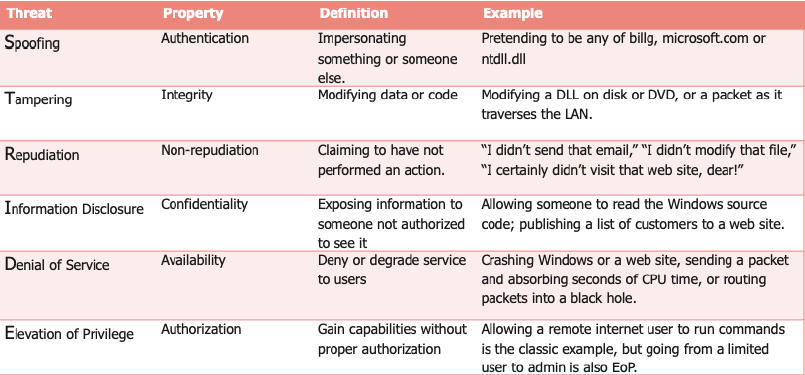
\includegraphics[width=1\linewidth]{../img/stride.png}
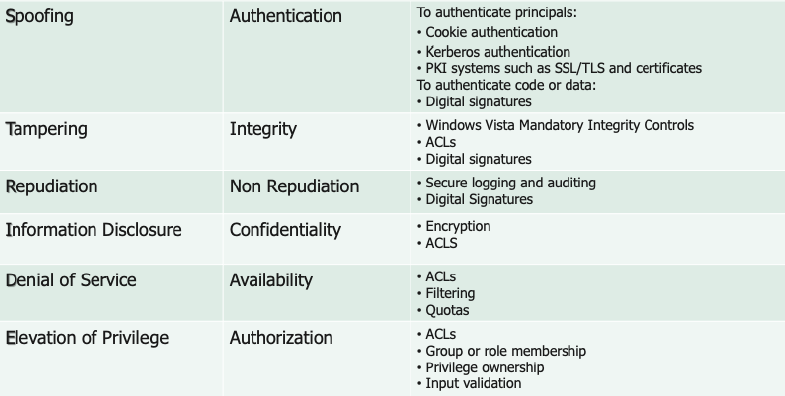
\includegraphics[width=1\linewidth]{../img/stride_mitigation.png}
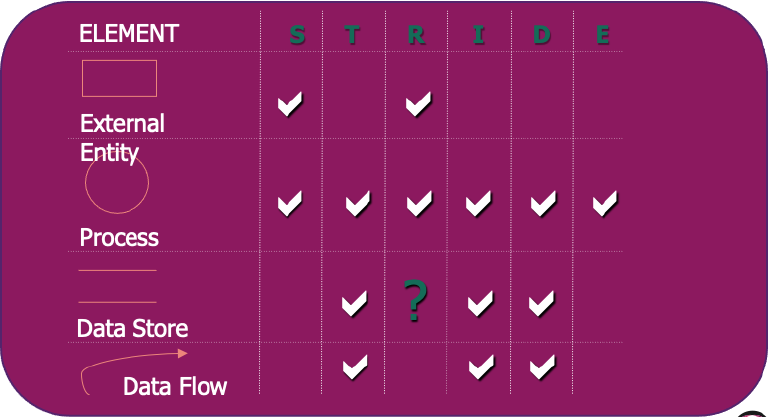
\includegraphics[width=1\linewidth]{../img/stride_mapping.png}\\
\columnbreak

\subsection{Attack Trees in context}
\begin{itemize}
    \item Very useful for developing one threat where mitigation is not obvious
    \item Complement a threat model
    \item Can start a threat modeling
    \item Can be used in teams
    \item Often generate good discussions
\end{itemize}


        %! Author = phili
%! Date = 28/06/2021

\section{Web Security}
\subsection{Introduction}
\begin{itemize}
    \item 56\% of internet traffic is automated (hacking tools etc.)
    \item Critical systems on the web
\end{itemize}
\subsection{OWASP}
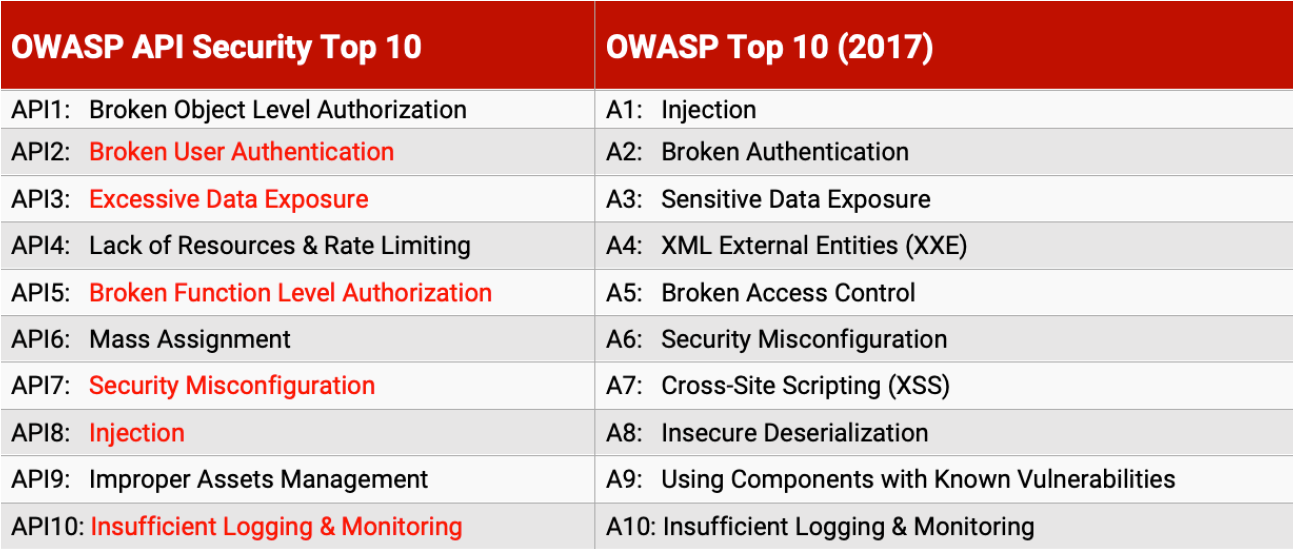
\includegraphics[width=\linewidth]{../img/owasp.png}

\subsection{Reasons for the many Security Incidents in the Web}
\begin{itemize}
    \item The way how we develop software (human errors)
    \item Almost no regulation
    \item Time to market (no time to update/fix/test)
    \item Not aware of the risk
    \item It's difficult
    \item Attractive for hackers, easy to access targets on the web
\end{itemize}

\subsection{XSS}
\begin{itemize}
    \item Client-side code injection attack (victim's browser)
    \item Executing malicious scripts in the victim's browser
    \item Vulnerable applications deliver malicious scripts
\end{itemize}

\includegraphics[width=0.7\linewidth]{../img/xss.pn.png}\\

\subsubsection{Stored XSS}
\begin{itemize}
    \item Script is permanently stored on the target server
    \item Malicious script is executed for every visitor
    \item \textbf{Typical Example:} Message board
\end{itemize}
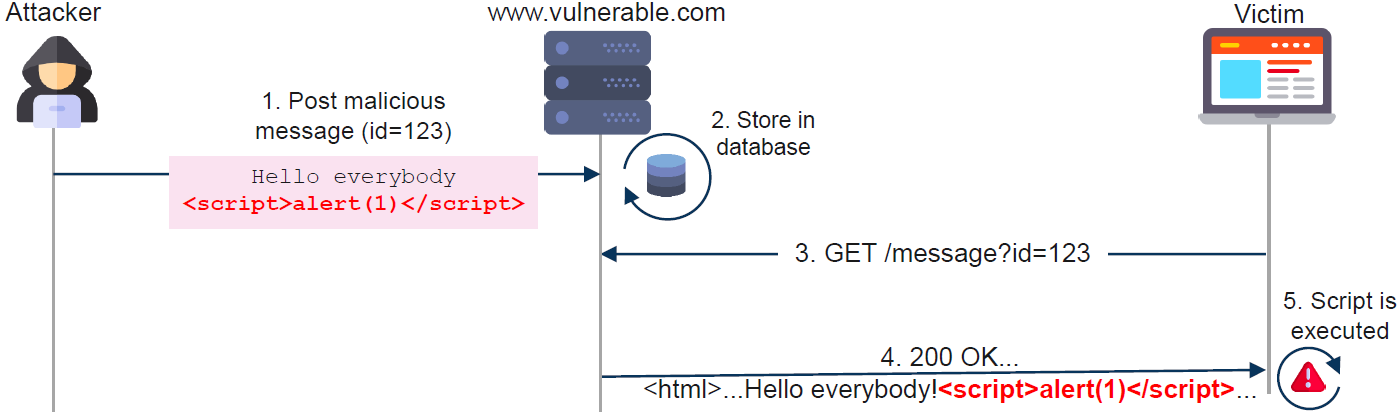
\includegraphics[width=\linewidth]{../img/xss_stored.png}
\textbf{Session Stealing Attack}\\
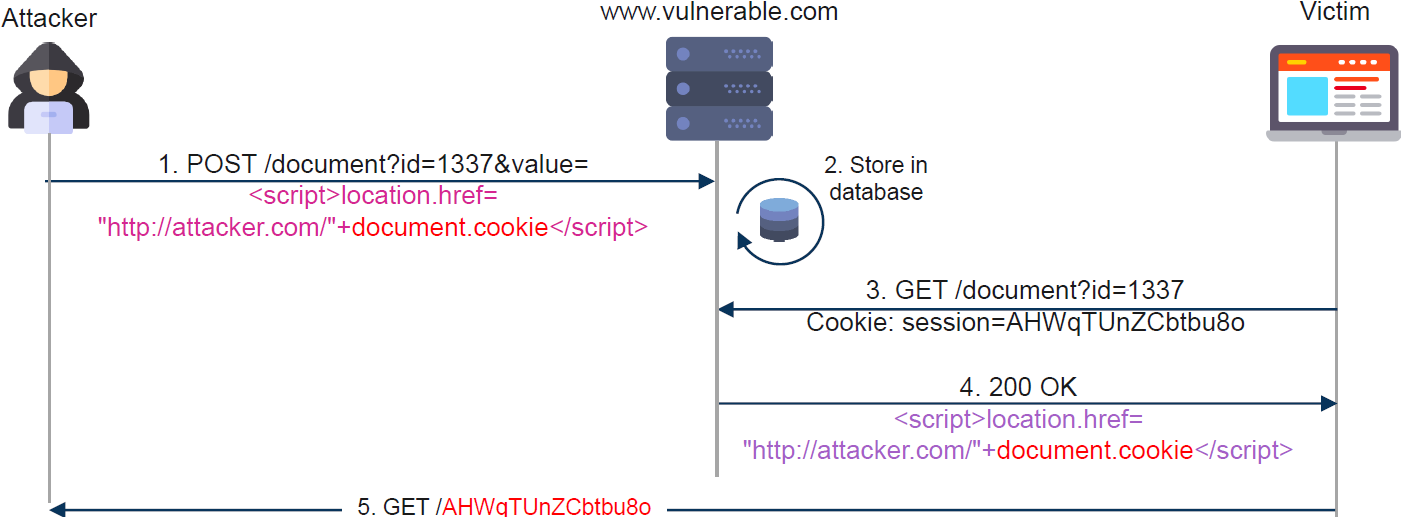
\includegraphics[width=\linewidth]{../img/xss_stored2.png}

\subsubsection{Reflected XSS}
\begin{itemize}
    \item Script is \textbf{not stored} on the target server
    \item Attacker usually needs to construct a malicious URL
    \item \textbf{Typical Example:} Search Form
\end{itemize}
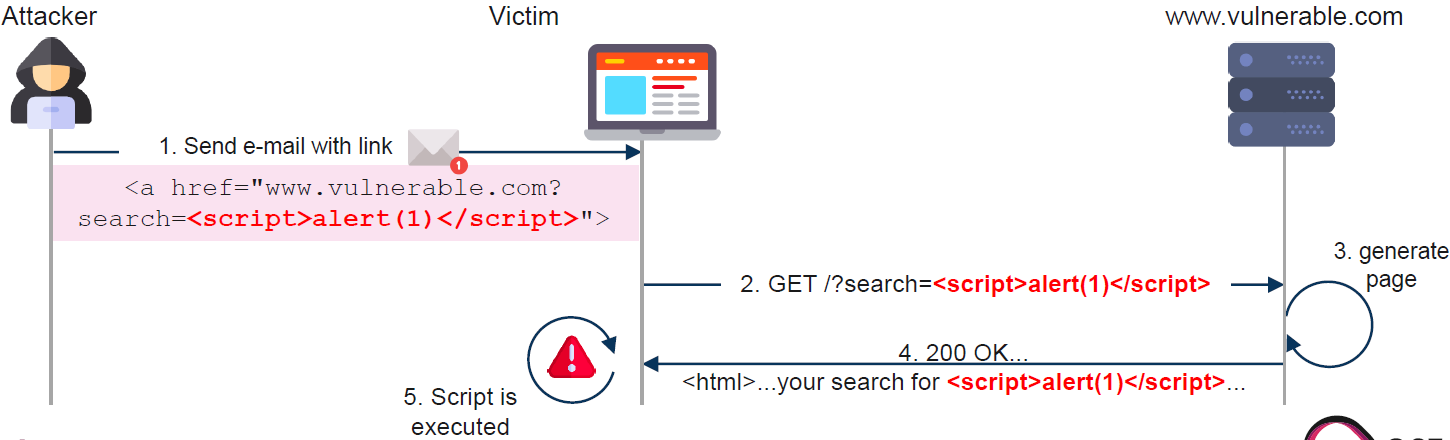
\includegraphics[width=\linewidth]{../img/xss_reflected.png}

\subsubsection{DOM based XSS}
\begin{itemize}
    \item Vulnerability is the client side code rather than server-side code
    \item Attacker needs to construct an URL
    \item Parameter of the URL is not processed by the server, but executed by the browser directly
\end{itemize}
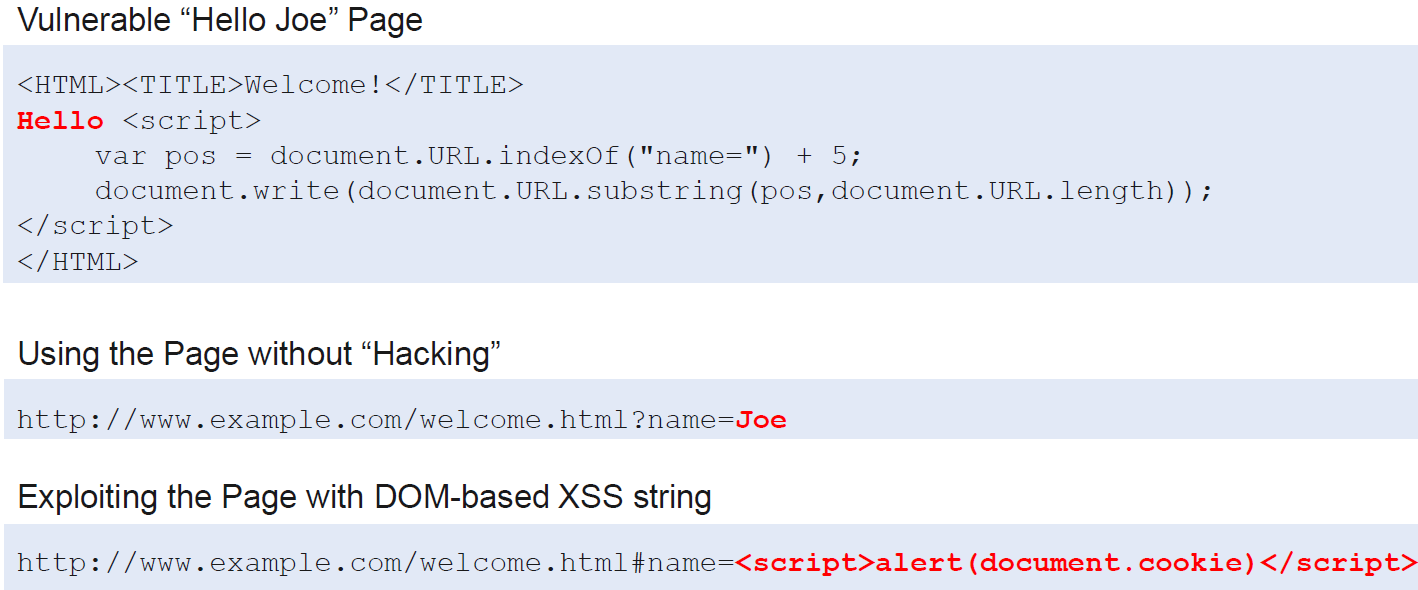
\includegraphics[width=\linewidth]{../img/xss_dom.png}

\subsubsection{Attack Vector Examples}
\begin{itemize}
    \item Script tags
    \item Event handler (\textit{onLoad, onClick} etc.)
    \item Links
    \item InnerHTML assignment (DOM-based XSS)
\end{itemize}

\subsubsection{Searching for XSS}
\begin{itemize}
    \item Play around with different strings in request params (script, \', \", etc.)
    \item In the page returned
    \begin{itemize}
        \item Search for the presence of test strings
        \item Check how the chars get filtered
        \item Find the problem and test with new strings
    \end{itemize}
\end{itemize}

\subsubsection{The power of \textless script src \textgreater}
\begin{itemize}
    \item Bypassing the SOP
\end{itemize}
\textbf{JavaScript from malware sites:}\\
JavaScript from www.attacker.com
IS \textbf{DENIED} from accessing resources
from www.vulnerable.com when the
JavaScript is loaded separately (e.g.
separate browser tab)\\
\textbf{Counter:}
JavaScript from www.attacker.com
IS \textbf{ALLOWED} to access resources
from www.vulnerable.com, if the
script is loaded by
www.vulnerable.com with
\textless script src="..."\textgreater

\subsubsection{XSS Protection}
\begin{itemize}
    \item Secure Programming
    \begin{itemize}
        \item Input / Output encoding of user supplied data (HTML entities)
        \item Input Validation (White/Blacklisting)
        \item Using XSS Protection Features in Frameworks
        \item Input sanitization of Web Frameworks
    \end{itemize}
    \item HTTP Response Header
    \item Cookie HttpOnly
    \begin{itemize}
        \item May prevent cookie / session stealing
        \item Malicious JavaScript can still \textbf{ride the session} and exfiltrate and manipulate the DOM
    \end{itemize}
    \item Browser XSS Filter (\textit{X-XSS-Protection: 1; mode=block})
    \begin{itemize}
        \item Asks Browser to render a blank page if XSS is detected
        \item Deprecated or never implemented for most browsers
        \item Poor detection rate
    \end{itemize}
    \item Content Security Policy (CSP)
    \begin{itemize}
        \item Firewall for the Browser
        \item Prevents code injection attacks like XSS
        \item Supported by modern browsers
        \item CSP defines, what is allowed to request from other domains
        \item CSP comes as http response header or HTML tag
    \end{itemize}
    \item Web Application Firewall
    \begin{itemize}
        \item WAF Input Validation
        \item Filtering HTTP Requests / Responses
        \item Searching for XSS Payload
    \end{itemize}
\end{itemize}

\subsection{Cross-Site Request Forgery}
\begin{itemize}
    \item End User executes unwanted actions while authenticated
\end{itemize}
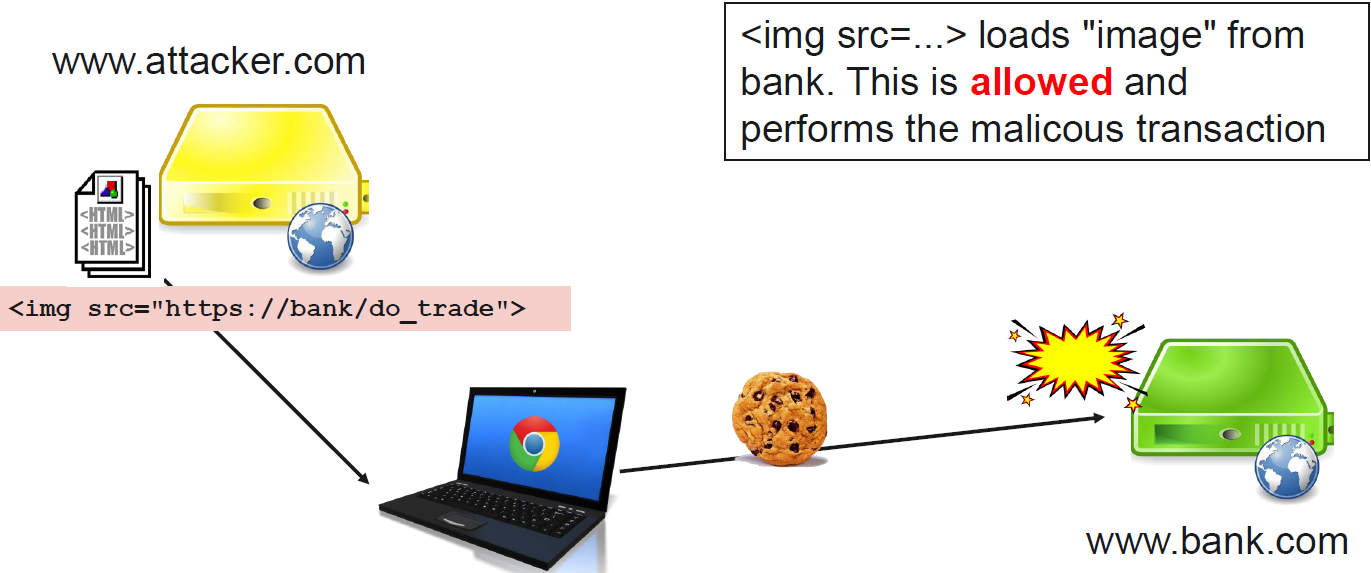
\includegraphics[width=\linewidth]{../img/xsrf.png}

\subsubsection{Pre-Requirement}
\begin{itemize}
    \item Know the target website / request
    \item Host the xsrf code somewhere
    \item Victim must have a valid session cookie
\end{itemize}

\subsubsection{XSRF Protection}
\begin{itemize}
    \item Random Token
    \begin{itemize}
        \item Form with a hidden field containing random token
    \end{itemize}
    \item SameSite Cookie Attribute
    \begin{itemize}
        \item Prevents browser from sending this cookie along with cross-site requests
        \item Mitigates cross-origin information leakage
        \item \textit{lax / strict}
    \end{itemize}
    \item CORS (only a mitigation)
    \begin{itemize}
        \item Configure CORS on the API service
        \item only allow requests from the fron-end origin
    \end{itemize}
    \item Framework Support
    \begin{itemize}
        \item AngularJS has built-in XSRF tokens on client side
        \item Server side must be implemented by the dev
    \end{itemize}
\end{itemize}

\subsection{HTTP Security Headers}
\textbf{Strict Transport Security}
\begin{itemize}
    \item HSTS
    \item \textit{Strict-Transport-Security: max-age=[ms]}
    \item Further requests in this time must occur over HTTPS
    \item Avoids all attacks based on HTTP downgrades
\end{itemize}
\textbf{X-Content-Type-Options}
\begin{itemize}
    \item nosniff
    \item Problem: Wrong Content-Type in HTTP Response
    \item e.g. Blocks a request if the requested type is \textit{style} and MIME type is not "text/css"
    \item Supported by all major browsers
\end{itemize}
\textbf{X-Frame-Options}
\begin{itemize}
    \item Prevent Website Framing
    \item Options: \textit{deny / SAMEORIGIN}
    \item Affects \textit{frame, iframe, embed, object}
\end{itemize}
\textbf{Referrer-Policy}
\begin{itemize}
    \item Control when URL information should be shared in the Referer header for other sites
    \item Options: \textit{no-referrer / same-origin / orign-when-cross-origin}
\end{itemize}
\textbf{Feature-Policy}
\begin{itemize}
    \item Allow and deny the use of browser features
\end{itemize}

\subsection{SQL Injection}
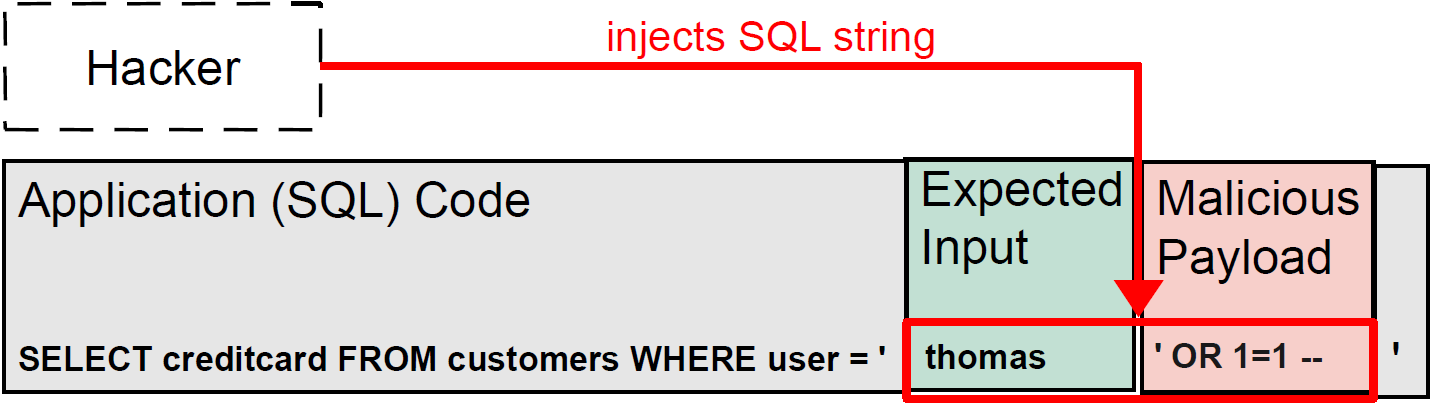
\includegraphics[width=\linewidth]{../img/sql_injection.png}
\subsubsection{Bypass Authentication}
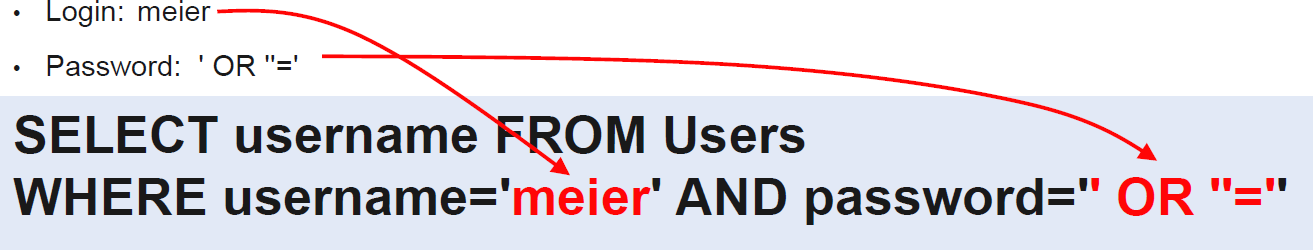
\includegraphics[width=\linewidth]{../img/sql_injection2.png}
\subsubsection{Fetch Arbitrary Information}
\begin{itemize}
    \item Access to System and catalog tables
\end{itemize}
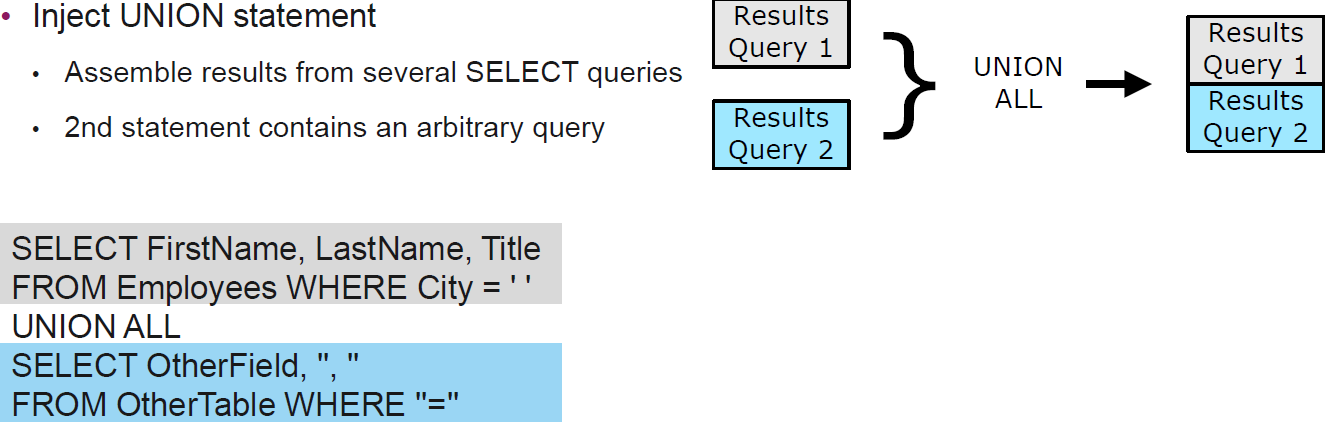
\includegraphics[width=\linewidth]{../img/sql_injection3.png}

\subsubsection{Hacking Database Example}
\begin{enumerate}
    \item What userID is running the MySQL database?
    \item Disclose Password hash from database
    \item Install Backdoor on Server through SQL Injection
    \item Upload more hacker tools on the server
\end{enumerate}

\subsubsection{Mitigation}
\begin{itemize}
    \item Secure Programming
    \begin{itemize}
        \item Prepared Statements / Stored Procedures
        \item Escaping
    \end{itemize}
    \item Error Handling
    \begin{itemize}
        \item Do not disclose details
    \end{itemize}
    \item Web Application Firewall
    \item DB least privileges
\end{itemize}

\subsection{XML External Entity Attack}
\subsubsection{XML Security}
\begin{itemize}
    \item XML signatures
    \item XML encryption
    \item XML key management
    \item Security Assertion Markup Language
    \item XML access control markup language
\end{itemize}

\subsubsection{Attack Vectors}
\textbf{XML Generator}\\
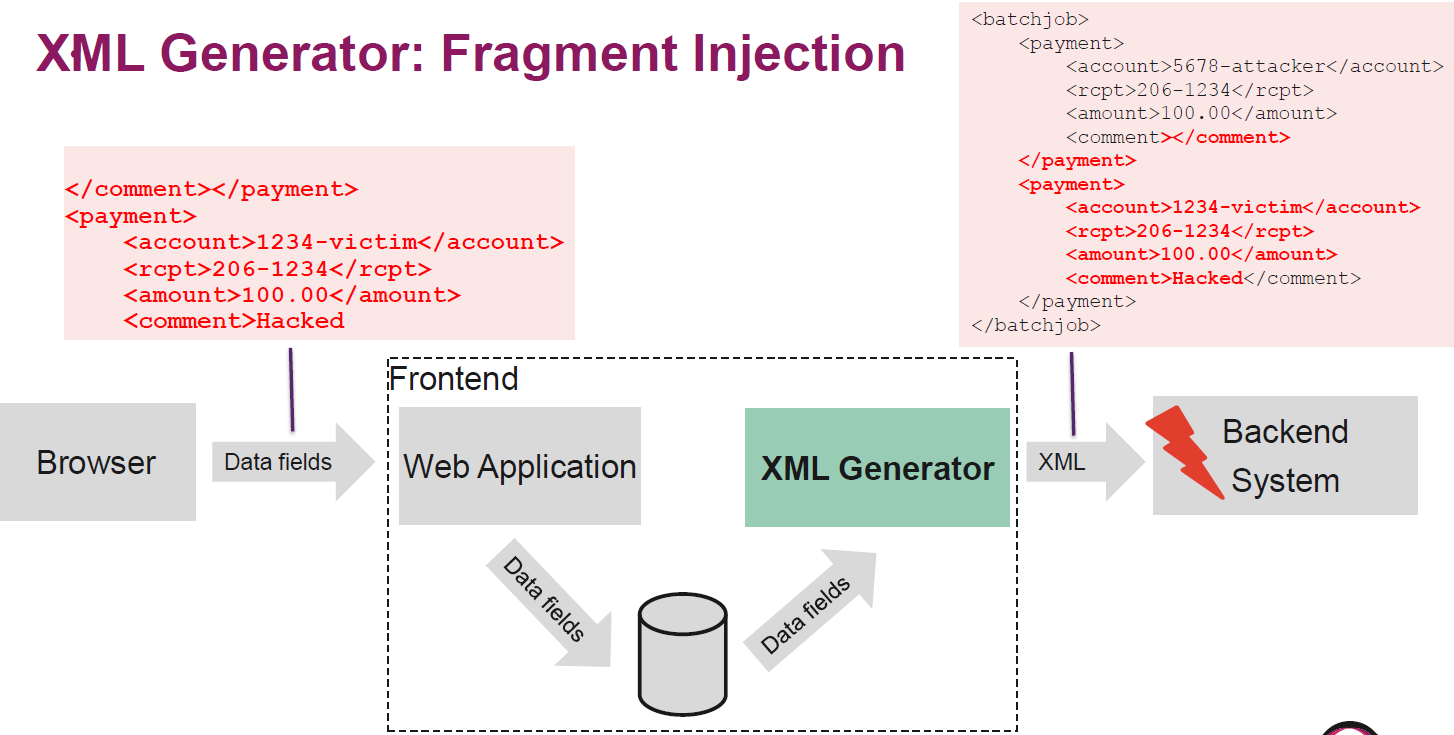
\includegraphics[width=\linewidth]{../img/xml_generator.png}
\textbf{Parser Attacks}
\begin{itemize}
    \item Attack Range
    \begin{itemize}
        \item DoS
        \item Inclusion of local files into XML documents (disclosure)
        \item Port scanning from the system where the parser is located
        \item Fetch data from local or remote systems
    \end{itemize}
\end{itemize}

\subsubsection{Mitigating XML Attacks}
\begin{itemize}
    \item Secure XML parser setup
\end{itemize}
        %! Author = phili
%! Date = 28/06/2021

\section{Bugs}
\textbf{Security Bug:}
\begin{itemize}
    \item Vulnerability at the implementation level
    \item Easy to discover / remediate using mondern code review tools
    \item E.g. buffer overflows, race conditions, unsafe system calls
\end{itemize}
\textbf{Security Flaw:}
\begin{itemize}
    \item Design level vulnerability
    \item Difficult / impossible to detect by automated tools
    \item Requires a manual risk analysis
    \item E.g. method overriding, error handling, type safety confusion
\end{itemize}
\textbf{Security Defect = Bug + Flaw}
\begin{itemize}
    \item Bugs / Flaws which may lie dormant for years
    \item Can surface in fielded systems with major consequences
\end{itemize}

\subsection{Example}
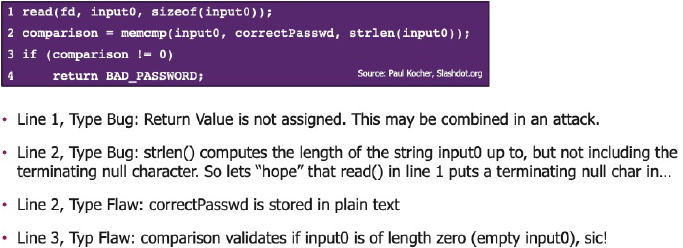
\includegraphics[width=\linewidth]{../img/bug_example.png}

\subsection{Memory Corruption}
\begin{itemize}
    \item Processes have their own address space others cant touch
    \item \textbf{Segmentation fault:} if a process tries to access memory outside its range
\end{itemize}

\subsubsection{Buffer Overflows}
\begin{lstlisting}
char buffer[4];
buffer[4] = 'a'; // Undefined behaviour
\end{lstlisting}
\begin{itemize}
    \item Can result in segmentation fault, if lucky
    \item Possible remote code execution, if unlucky
\end{itemize}
\textbf{Solution:}
\begin{itemize}
    \item Check array boundary at runtime
\end{itemize}

\subsubsection{Other memory corruption issues}
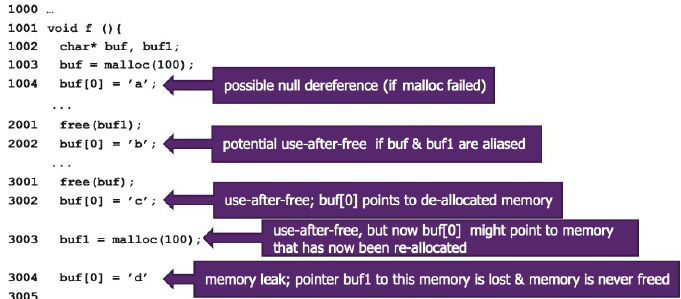
\includegraphics[width=\linewidth]{../img/memory_corruptions.png}

\subsection{Buffer Overflow}
\subsubsection{Process Memory Layout}
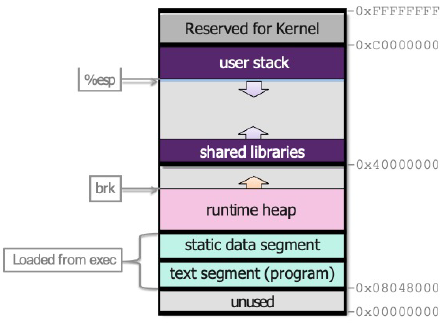
\includegraphics[width=0.6\linewidth]{../img/process_memory_layout.png}
\subsubsection{Stack Frame}
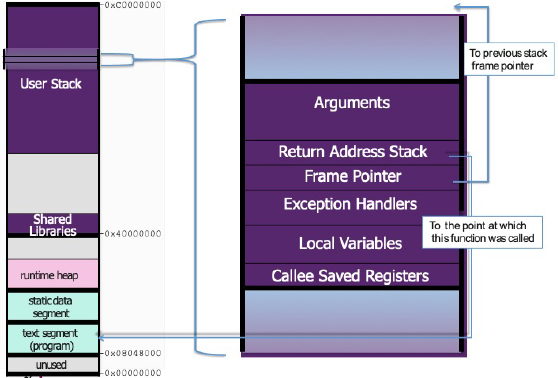
\includegraphics[width=0.6\linewidth]{../img/stack_frame.png}
\subsubsection{Problematic libc functions}
\begin{itemize}
    \item strcpy
    \item strcat
    \item gets
    \item scanf
\end{itemize}
\textbf{Safe versions:}
\begin{itemize}
    \item strncpy
    \item strncat
\end{itemize}

\subsubsection{Defenses}
\textbf{Compile:}\\
Harden programs to resist attacks in new programs.\\
\begin{itemize}
    \item Use a modern Programming Language
    \item Safe Coding Techniques
    \item Language Extensions / Safe Libraries
    \item Stack protection
    \begin{itemize}
        \item Canaries: Check function entry and exit code to check for corruption
        \item Random / Terminate canary
    \end{itemize}
\end{itemize}
\textbf{Run:}\\
Aim to detect and abort attacks in existing programs.\\
\begin{itemize}
    \item Executable Address Space Protection
    \begin{itemize}
        \item Use virtual memory support to make some regions of memory non-executable
    \end{itemize}
    \item ASLR: Address Space Layout Randomisation
    \item Non Executable Memory
\end{itemize}

\subsection{Race Condition}
\begin{itemize}
    \item Concurrency can lead to nondeterministic behaviour
    \item Software defects resulting from unanticipated execution ordering
    \item Necessary properties
    \begin{itemize}
        \item Concurrency
        \item Shared object
        \item Change state
    \end{itemize}
\end{itemize}

\subsubsection{Race Window}
\begin{itemize}
    \item Occurs in a code segment that accesses the race object
    \item Window of opportunity for race condition
    \item Critical Section
\end{itemize}

\subsubsection{Time of Check and Time of Use (ToCToU)}
\begin{itemize}
    \item Can occur during file I/O
    \item Forms a Race Window by first checking some race object and then using it
\end{itemize}
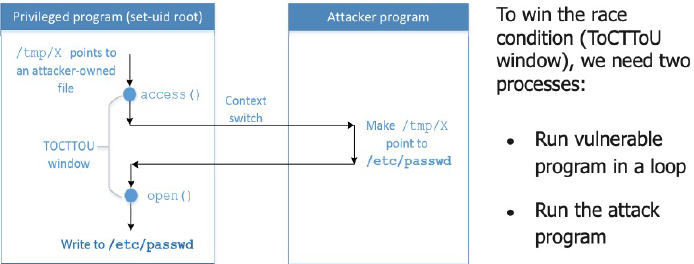
\includegraphics[width=\linewidth]{../img/toctou.png}

\subsubsection{How to Exploit Race Condition}
\begin{enumerate}
    \item Choose a target file (e.g. \textit{/etc/passwd})
    \item Launch Attack
    \begin{itemize}
        \item Attack Process
        \item Vulnerable Process
    \end{itemize}
    \item Monitor the result (check timestamp)
    \item Run the exploit
\end{enumerate}

\subsubsection{Mitigations}
\begin{itemize}
    \item Atomic Operations
    \item Repeating Check and Use
    \item Sticky Symlink Protection
    \item Principles of Least Privilege
\end{itemize}
        \usepackage{listings}
\usepackage{graphicx}%! Author = phili
%! Date = 28/06/2021

\section{Integer Security}
\begin{itemize}
    \item Integer boundary concerns are often ignored
    \item Ariane 5 destroyed after integer overflow
    \item Results of integer overflow depend on the language and hardware
\end{itemize}
\textbf{Integer Promotion Example:}
\begin{lstlisting}
char c1, c2;
c1 = c1 + c2;
\end{lstlisting}

\subsection{Implicit Conversions}
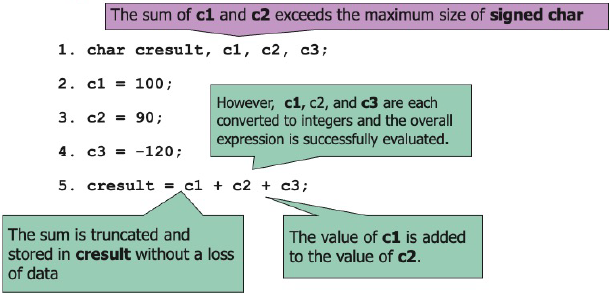
\includegraphics[width=\linewidth]{../img/implicit_conversions.png}

\subsection{Signed Integer Conversion}
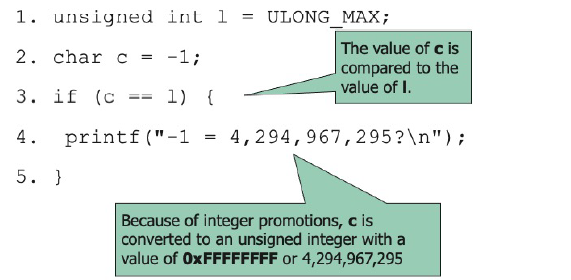
\includegraphics[width=\linewidth]{../img/signed_integer_conversion.png}

\subsection{Overflow Examples}
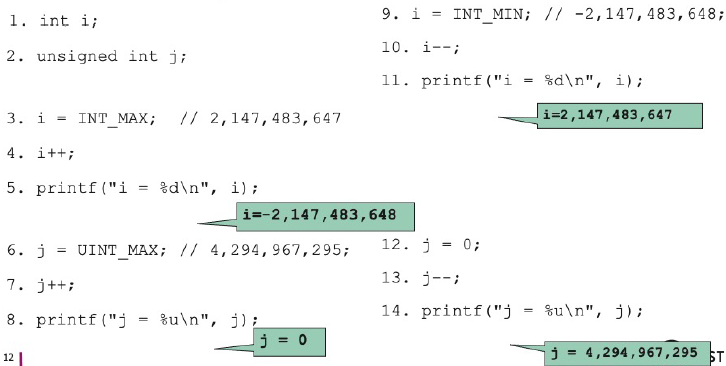
\includegraphics[width=\linewidth]{../img/overflow_examples.png}

\subsection{Truncation Error Example}
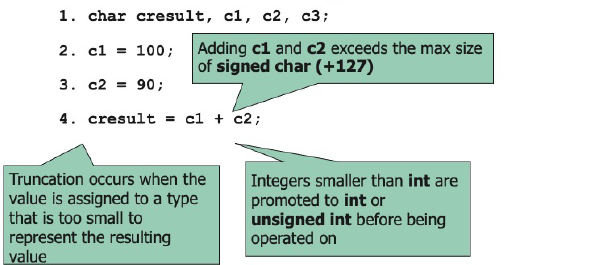
\includegraphics[width=\linewidth]{../img/truncation_error.png}
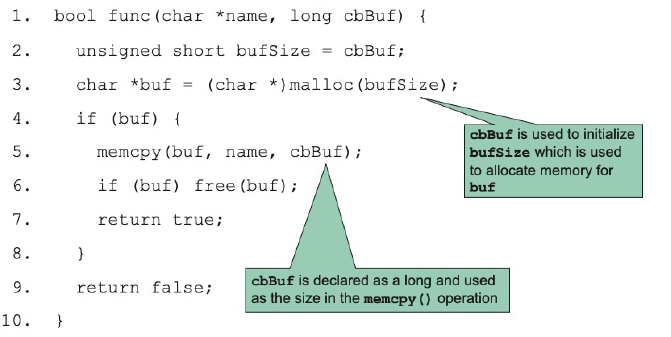
\includegraphics[width=\linewidth]{../img/truncation_error2.png}

\subsection{Sign Error Example}
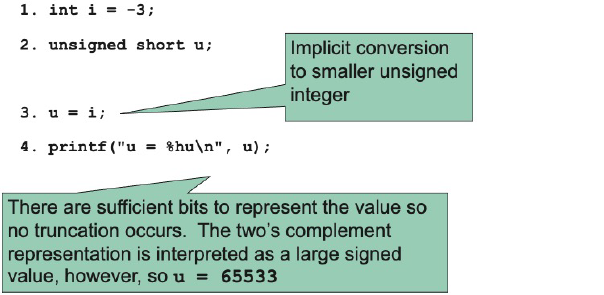
\includegraphics[width=\linewidth]{../img/sign_error.png}
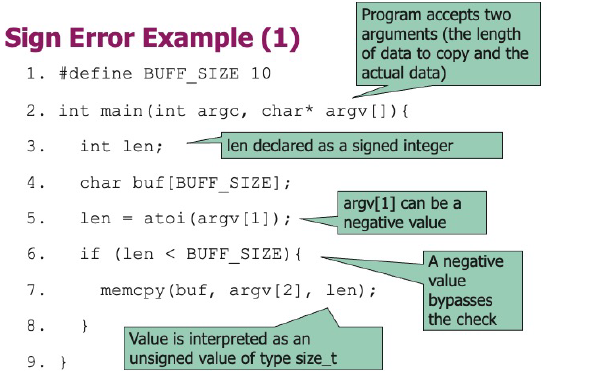
\includegraphics[width=\linewidth]{../img/sign_error2.png}

\subsection{Integer Division}
\begin{itemize}
    \item Minimum integer value divided by $-1$
    \item $-2'147'483'648 / -1 = -2'147'483'648$
\end{itemize}

\subsection{Negative Indices}
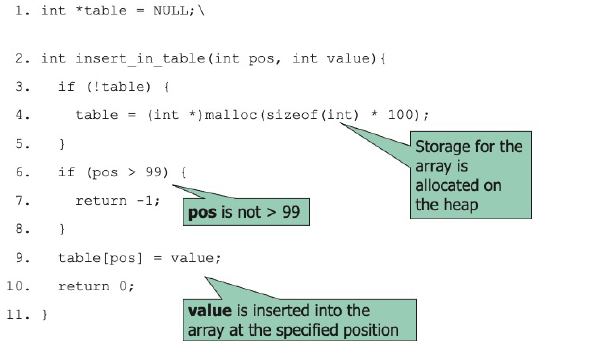
\includegraphics[width=\linewidth]{../img/negative_indices.png}

\subsection{Mitigation}
\textbf{Strong Typing}
\begin{itemize}
    \item Provide better types
    \item Using unsigned type to guarantee positive values
    \item Does not prevent overflow
\end{itemize}
\textbf{Abstract Data Type}
\begin{itemize}
    \item Create an abstract data type with private variables
    \item User can only changes values using public method calls
    \item Methods check valid range of input
\end{itemize}
\textbf{Safe Int Class}
\begin{itemize}
    \item C++ template class
    \item Tests the values of operands before performing an operation
\end{itemize}
\textbf{Testing}
\begin{itemize}
    \item Boundary checks
\end{itemize}
\textbf{Source Code Audit}
\begin{itemize}
    \item Source code should be audited or inspected
\end{itemize}
        %! Author = Philipp Emmenegger
%! Date = 29/06/2021

\section{Reverse Engineering}
Software Reverse Engineering helps:
\begin{itemize}
    \item understand malware
    \item understand legacy code
    \item remove usage restriction from software
    \item fond and exploit flaws 
    \item cheat at games
\end{itemize}

\subsection{Compiling}
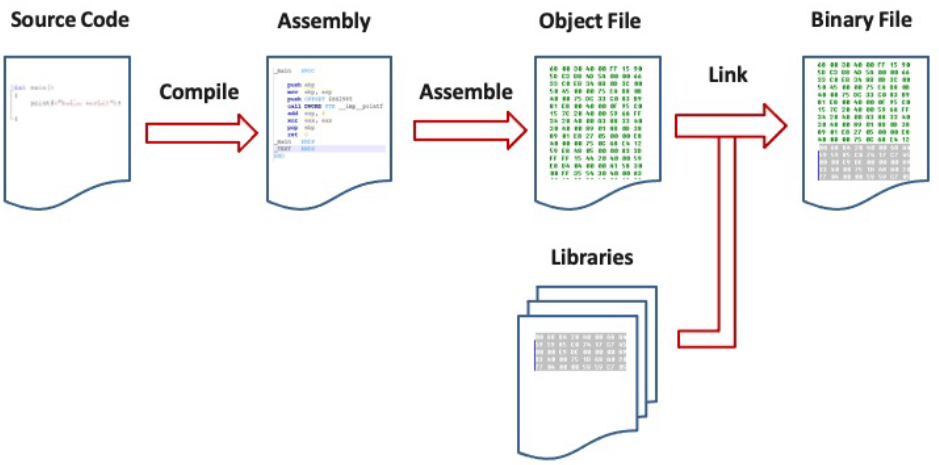
\includegraphics[width=\linewidth]{../img/compiling.png}

\subsection{Loading}
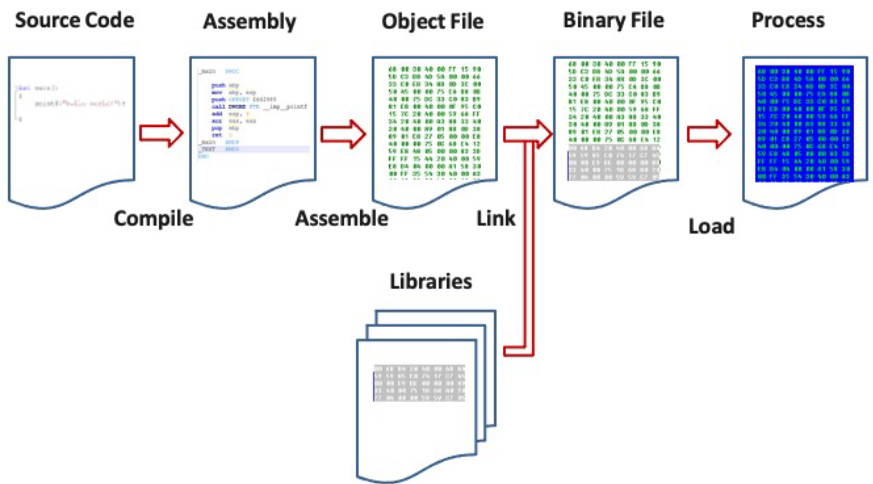
\includegraphics[width=\linewidth]{../img/loading.png}

\subsection{Running}
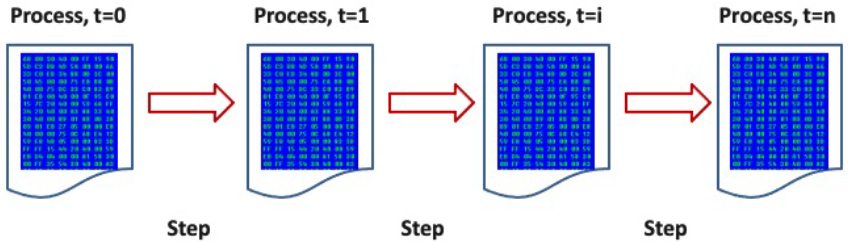
\includegraphics[width=\linewidth]{../img/running.png}

\subsection{Reverse Engineering Domain}
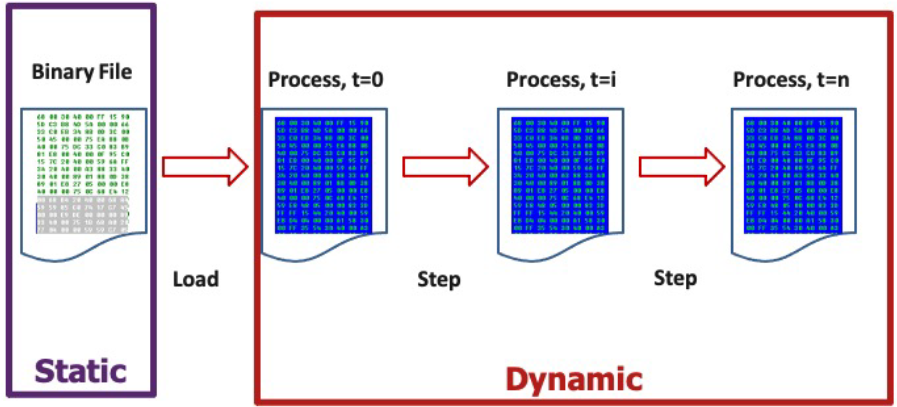
\includegraphics[width=\linewidth]{../img/reverse_engineering_domain.png}

\subsection{Tools}
\textbf{Disassembler}
\begin{itemize}
    \item Converts exe to assembly (as best as it can)
    \item Cannot always disassemble 100\% correctly
    \item Not possible to reassemble into working exe
    \item Gives static results
    \item Good overview of program logic
    \item Difficult to jump to specific place in the code
\end{itemize}
\textbf{Debugger}
\begin{itemize}
    \item Step thru code to understand it
    \item Labor intensive
    \item Can set break points
    \item Can treat complex code as black box
\end{itemize}
\textbf{Hex editor}
\begin{itemize}
    \item Patch (modify) exe file
\end{itemize}
\textbf{Process Monitor, VMware, ...}

\subsection{Mitigations against Reverse Engineering}
\begin{itemize}
    \item Impossible to prevent
    \item Possible to make it more difficult
    \begin{enumerate}
        \item Anti-disassembly: confuse static view of code
        \item Anti-debugging: confuse dynamic view of code
        \item Tamper resistance: code checks itself to detect tampering
        \item Code obfuscation: make code more difficult to understand
    \end{enumerate}
\end{itemize}

\subsubsection{Anti Dissasembly}
\begin{itemize}
    \item Encrypted or packed object code
    \item False disassembly
    \item Self-modifying code
    \item Encryption prevents disassembly
\end{itemize}

\subsubsection{Anti Debugging}
\begin{itemize}
    \item \textit{IsDebuggerPresent()}
    \item Monitor for debug registers / breakpoints
    \item Debuggers do not handle threads well
\end{itemize}
\textbf{Example:}
\begin{itemize}
    \item Programs gets \textit{inst 1} and pre fetches following
    \item Debugger does not pre-fetch
    \item Overwrite later instruction after pre fetching
    \item Program without debugger will be okay
    \item Only works if segment of code is executed once
\end{itemize}

\subsubsection{Tamper Resistance}
\begin{itemize}
    \item Make patching more difficult
    \item Code can hash parts of itself, hash checks later
    \item This approach is called \textit{guards}
\end{itemize}

\subsubsection{Code Obfuscation}
\begin{itemize}
    \item Make code hard to understand
    \item Opposite of good software engineering
    \item spaghetti code
\end{itemize}
\begin{lstlisting}
int x,y;
if((x-y)*(x-y) > (x*x-2*x*y+y+y)) { } // always true
\end{lstlisting}
\textbf{Code Bloating:}
\begin{enumerate}
    \item Insert dead code
    \item Adding zero effect operations
    \item Transform the data (ASCII Chars instead of numbers)
\end{enumerate}
        %! Author = Philipp Emmenegger
%! Date = 29/06/2021

\section{Assurance}
Confidence that an entity meets its security requirements based on evidence provided by applying assurance techniques.\\
\textbf{Trusted System:}
\begin{itemize}
    \item Meets well defined requirements
    \item Evaluated by a credible body of experts
    \item Use specific methodologies to gather evidence
\end{itemize}

\subsection{Issues with one-time evaluations}
\begin{enumerate}
    \item Requirements definitions may be flawed
    \item System design can be flawed
    \item Hardware implementation maybe faulty
    \item Software implementation: well, errors, bugs
    \item System use and operation errors
    \item Willful system misuse
    \item Hardware, communication or other equipment malfunction
    \item Environmental problems
    \item Evolution, maintenance, faulty upgrades and decomissions
\end{enumerate}

\subsection{Types of Assurance}
\textbf{Policy Assurance:}\\
Evidence establishing security requirements in policy is complete, consistent, technically sound.\\
\textbf{Design Assurance:}\\
Evidence establishing design sufficient to meet requirements of security policy.\\
\textbf{Implementation Assurance:}\\
Evidence establishing implementation consistent with security requirements of security policy.\\
\textbf{Operational Assurance:}\\
Evidence establishing system sustains the security policy requirements during installation, configuration and day-to-day operation.

\subsection{Assurance in Software Development LiveCycle (SDLC)}
\textbf{Conception}
\begin{itemize}
    \item Decision to pursue it
    \item Proof of concept to see if idea has merit
    \item High level requirements analysis
    \item Identify threats, assumptions
\end{itemize}
\textbf{Manufacture}
\begin{itemize}
    \item Develop detailed plans for each group involved
    \item Implement the plans to create entity
\end{itemize}
\textbf{Deployment}
\begin{itemize}
    \item Delivery Assure that correct masters are delivered to production
    \item Assure integrity of what is delivered to customers
\end{itemize}
\textbf{Fielded Product Life}
\begin{itemize}
    \item Routine Maintenance
    \item Patching
    \item Support
    \item Decomissoning
\end{itemize}

\subsection{Evaluation Models}
\subsubsection{Orange Book (TCSEC)}
Collection of criteria used to grade or rate the security offered by a computer system product.\\
\textbf{C1: Discretionary Protection}
\begin{itemize}
    \item Identification
    \item Authentication
    \item Discretionary access control
\end{itemize}
\textbf{C2: Controlled Access Protection}
\begin{itemize}
    \item Object reuse and auditing
\end{itemize}
\textbf{B1: Labled security protection}
\begin{itemize}
    \item Mandatory access control on limited set of objects
    \item Informal model of the security policy
\end{itemize}
\textbf{B2: Structured Protections}
\begin{itemize}
    \item Trusted path for login
    \item Principle of least privilege
    \item Formal model of Security Policy
    \item Covert channel analysis
    \item Configuration management
\end{itemize}
\textbf{B3: Security Domains}
\begin{itemize}
    \item Full reference validation mechanism
    \item Constraints on code development process
    \item Documentation, testing requirements
\end{itemize}
\textbf{A: Verified Protection}
\begin{itemize}
    \item Formal methods for analysis, verification
    \item Trusted distribution
\end{itemize}

\subsubsection{TCSEC Evaluation}
\textbf{Three Phases}
\begin{itemize}
    \item Design analysis
    \item Test analysis
    \item Final Review
\end{itemize}
\textbf{Issues:}
\begin{itemize}
    \item Based heavily on confidentiality
    \item Not addressing integrity / availability
    \item Tied security and functionality together
\end{itemize}

\subsubsection{Common Criteria (CC)}
\begin{itemize}
    \item Provides IT security requirements for IT products
    \item Provides metric to quantify level of security
    \item Addressed Requirements:
    \begin{itemize}
        \item Functional: define desired security behaviour
        \item Assurance: indicating claimed security measures are effective and implemented correctly
    \end{itemize}
\end{itemize}
\textbf{Purpose:}
\begin{itemize}
    \item Provide consistent evaluation standards
    \item Improve the availability of evaluated systems
    \item Eliminate duplicating evaluations
    \item Improve the efficiency and cost-effectiveness
\end{itemize}

\subsubsection{CC Process Approach}
\textbf{Target of Evaluation (ToE):}\\
Name of the specific item that is the subject of the security evaluation.\\
\textbf{Security Target (ST):}\\
Standard used for the evaluation.\\
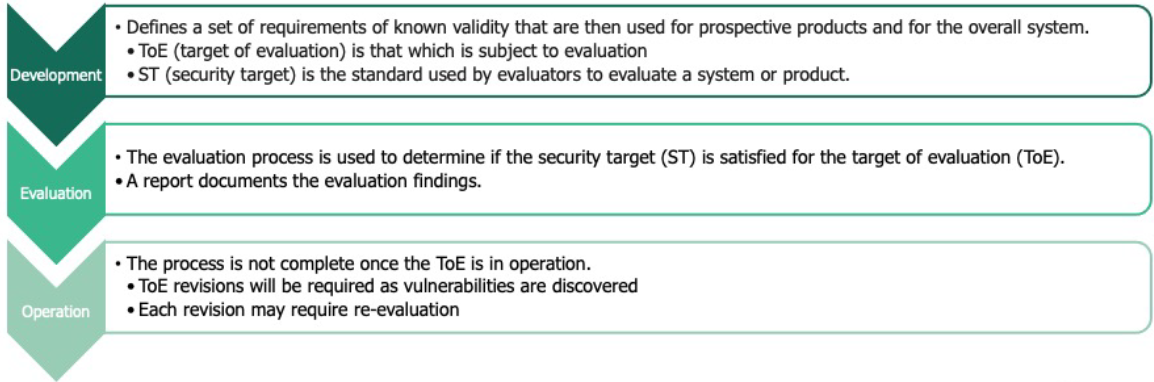
\includegraphics[width=\linewidth]{../img/common_criteria.png}
\textbf{Assurance Levels (EAL:}\\
\begin{itemize}
    \item EAL 1: Functionally tested
    \item EAL 2: Structurally tested
    \item EAL 3: Methodically tested and Checked
    \item EAL 4: Methodically Designed, Tested and Reviewed
    \item EAL 5: Semiformal Designed, and Tested
    \item EAL 6: Semiformal Verified Design and Tested
    \item EAL 7: Formally Verified Design and Tested
\end{itemize}

\columnbreak
\subsubsection{CC Evaluation}
\begin{enumerate}
    \item Protection Profile
    \begin{itemize}
        \item Implementation independant, domain specific set of security requirements
    \end{itemize}
    \item Security Target
    \begin{itemize}
        \item Specific requirements used to evaluate system
    \end{itemize}
\end{enumerate}

\subsubsection{Example Threat in CC}
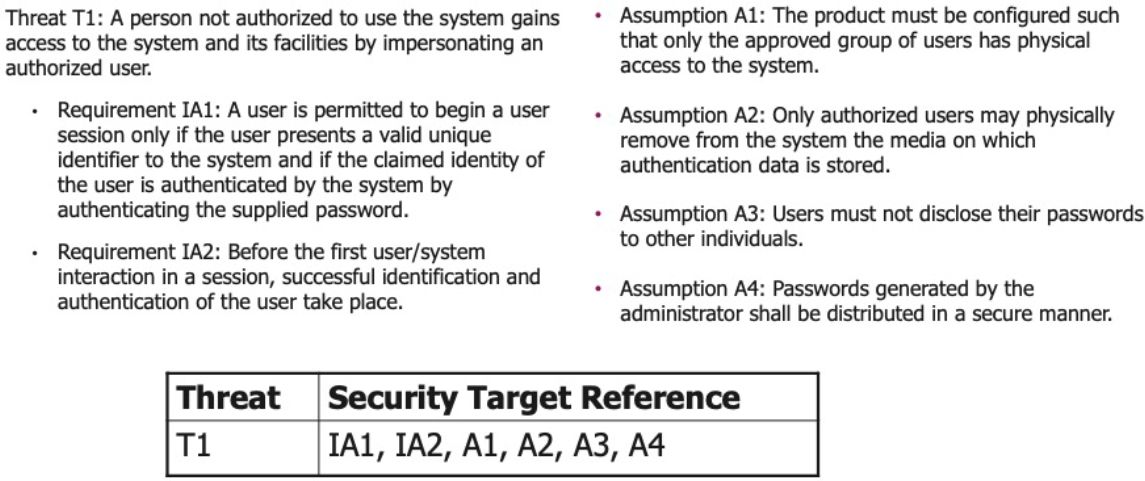
\includegraphics[width=\linewidth]{../img/example_threat_cc.png}
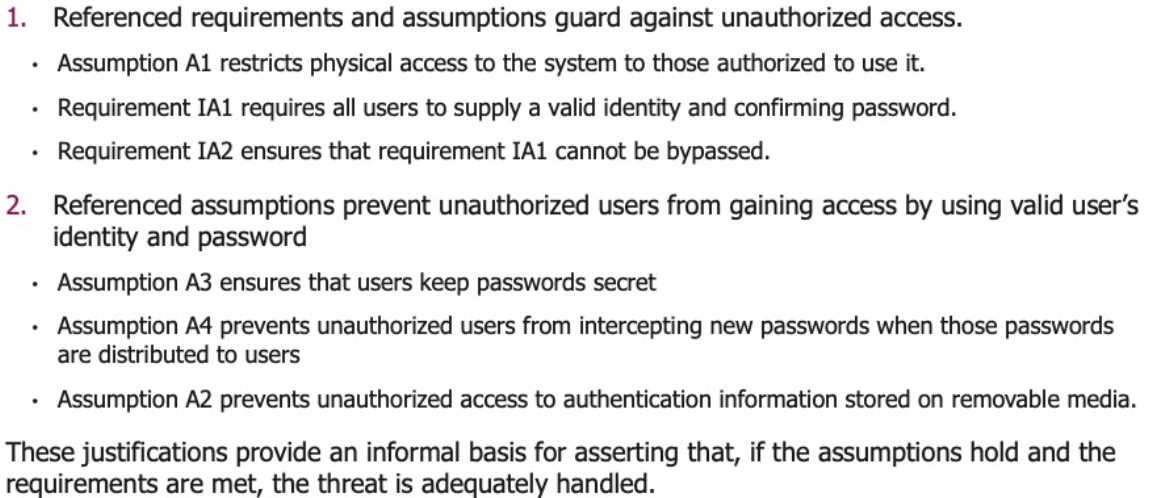
\includegraphics[width=\linewidth]{../img/example_threat_cc2.png}

\subsection{Security Target}
\subsubsection{PP/ST Framework}
\begin{itemize}
    \item Product Approach usually for STs
    \item Define what product does
    \item Define existing documentation/assurance
\end{itemize}
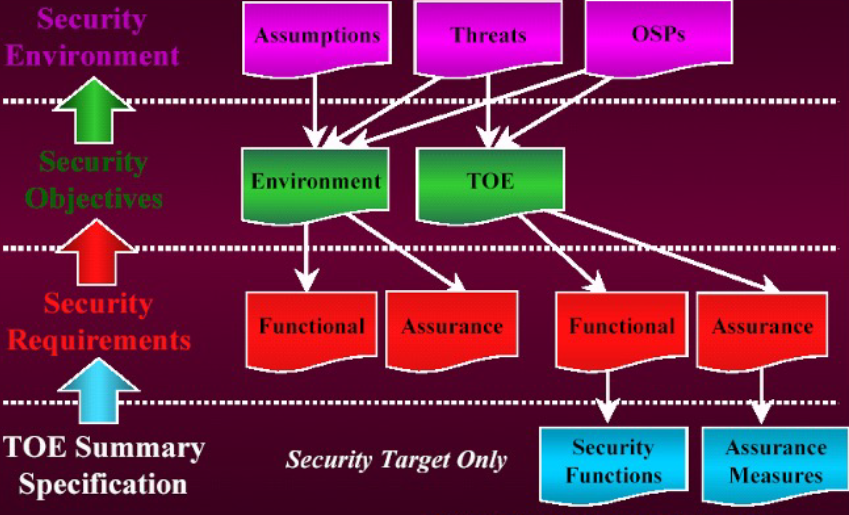
\includegraphics[width=0.5\linewidth]{../img/pp_st_framework.png}
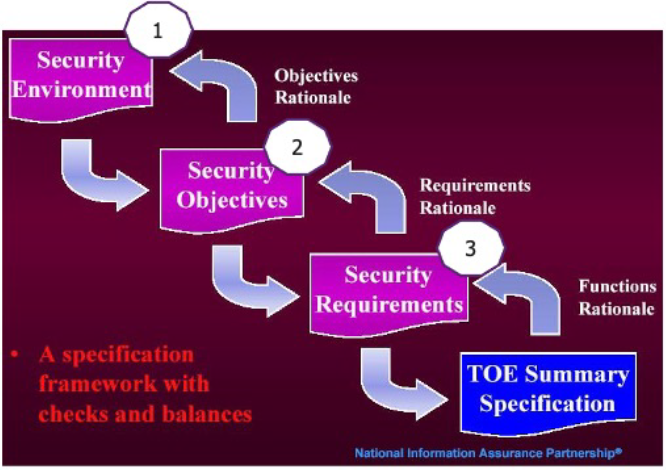
\includegraphics[width=0.5\linewidth]{../img/pp_st_framework2.png}

\subsubsection{Security Environment}
\begin{itemize}
    \item \textbf{Secure usage Assumptions} aspects of the environment intended to use
    \item Describes the security aspects
    \item \textbf{Threats:} The ability to exploit a vulnerability by a threat agent
    \item \textbf{Organizational Security Policies:} Set of rules, procedures, practices imposed by an organization
\end{itemize}

\subsubsection{Security Requirements}
\textbf{Functional Requirements}
\begin{itemize}
    \item Defining security behaviour
    \item Implemented requirements become security functions
    \item Examples:
    \begin{itemize}
        \item Identification / Authentication
        \item Audit
        \item User Data protection
    \end{itemize}
\end{itemize}
\textbf{Assurance Requirements}
\begin{itemize}
    \item Establishing confidence in security functions
    \begin{itemize}
        \item Correctness of implementation
        \item Effectiveness in satisfying security objectives
    \end{itemize}
    \item Examples:
    \begin{itemize}
        \item Development
        \item Configuration Management
        \item Life Cycle Support
        \item Testing
    \end{itemize}
\end{itemize}

\subsubsection{Reading Guidance}
\begin{itemize}
    \item Class: Differ in coverage of security objectives
    \item Family: Differ in rigor or emphasis
    \item Component: Describes an actual set of security requirements
    \item Element: Members of a component
\end{itemize}
\includegraphics[width=0.6\linewidth]{../img/reading_guidance.png}

\subsubsection{Security Functionality Classes}
\includegraphics[width=\linewidth]{../img/security_functionality_classes.png}

\subsection{Design Document}
\begin{itemize}
    \item Provide basis for analysis
    \begin{itemize}
        \item Informal
        \item Semiformal
        \item Formal
    \end{itemize}
    \item Must include:
    \begin{itemize}
        \item Security Functions
        \item External Interfaces
        \item Internal Design
    \end{itemize}
\end{itemize}

\subsubsection{Security Functions}
\begin{itemize}
    \item Identifies high-level security functions defined for the system
    \item Includes:
    \begin{itemize}
        \item Description of individual functions
        \item Overview of set of security functions, how they work together
        \item Mapping of requirements, mapping functions to requirements
    \end{itemize}
\end{itemize}

\subsubsection{External Interfaces}
High level description of external interfaces to system, component, subcomponent or module
\begin{enumerate}
    \item \textbf{Component overview}: Identifying the component, its parent, how it fits into the design
    \item \textbf{Data descriptions:} Identifying data types and structures needed to support the external interface
    \item \textbf{Interface descriptions}
\end{enumerate}
\includegraphics[width=\linewidth]{../img/external_interface.png}

\subsubsection{Internal Design}
Describes internal structures and functions of components of system.
\begin{enumerate}
    \item Overview of the parent component
    \item Detailed description of the component
    \item Security relevance of the component
\end{enumerate}

\subsection{Activities done to gain assurance}
\begin{enumerate}
    \item Analysis of the correspondence between TOE design representations
    \item Analysis of the TOE design representations against the requirements
    \item Analysis of functional tests coverage and results
    \item Independent functional testing
    \item Penetration testing
    \item Verification of mathematical proofs
    \item Analysis of guidance documents
    \item Analysis of processes and procedures
    \item Checking that processes and procedures are being applied
\end{enumerate}
        %! Author = Philipp Emmenegger
%! Date = 29/06/2021

\section{Security Testing}
Process intended to reveal flaws in the security mechanisms.\\
\includegraphics[width=\linewidth]{../img/security_testing.png}

\subsection{Verification in SDLC}
\includegraphics[width=\linewidth]{../img/verification_sdlc.png}

\subsection{Measurement Terminology}
\includegraphics[width=\linewidth]{../img/measurement_terminology.png}
\textbf{Issues:}
\begin{itemize}
    \item Too many false positives: Tool wasted my time
    \item Too many false negatives: Tool missed the important
\end{itemize}

\subsection{Application to (Static) Application Security Testing Tools}
\includegraphics[width=\linewidth]{../img/application.png}

\columnbreak
\subsection{Static Analysis Tools}
\subsubsection{Static Application Security Testing (SAST)}
\begin{itemize}
    \item Based on white-hat / white-box
    \item Tester knows information about the system
    \item Examine source code at rest to detect and report security weaknesses
    \item Some tools run on source code, some on compiled code, some on both
\end{itemize}
\textbf{Functional Components of a SAST Tool}\\
\includegraphics[width=\linewidth]{../img/sast_tool.png}\\
\textbf{Data Flow Analysis Techniques compiled into SAST}
\begin{enumerate}
    \item Control Flow Graph: Follow the control flow to identify dangerous sequences
    \item Tainting Analysis: Identify variable that have been tainted with user input, follow them if passed without sanitization
    \item Lexical Analysis: Tokenize source code to make it easier to analyse
\end{enumerate}

\subsection{Dynamic Analysis Tools}
\subsubsection{Web Application Scanners}
\begin{itemize}
    \item Pretend Browser
    \item Goes through the various web forms and links
    \item Sends in attack-like and random data, tries to detect problems
    \item Easy and quick to use
    \item OWASP ZAP
\end{itemize}

\subsubsection{Fuzzing}
\begin{itemize}
    \item Provide a large number of random inputs
    \item Monitor program results and not if the final answer is correct
    \begin{itemize}
        \item Crashes
        \item Fails code assertions
        \item Memory leaks
    \end{itemize}
\end{itemize}

\subsubsection{Test Data Creation Techniques}
\begin{enumerate}
    \item Black Box (fully random): Feed the program random inputs. Very easy but rather inefficient
    \item Mutation based: Mutate input samples to create test data
    \item Generation based: Create test data based on model of input
\end{enumerate}
\textbf{Imporvements:}
\begin{itemize}
    \item Constraints: Generating tests that execute previously unused code paths
    \item Heuristics: Create likely security vulnerability patterns
    \item Variate on the type of input data
\end{itemize}

\subsection{Code Coverage}
\begin{itemize}
    \item \textbf{Statement coverage:} Which percentage of statements have been executed
    \item \textbf{Branch coverage:} Which percentage of branch options have been executed
\end{itemize}

\subsection{Software Composition Analysis (SCA)}
\begin{itemize}
    \item Historically developed to check legal status of embedded software libraries
    \item Today: powerful tool to get inside about the propagation of vulnerabilities in 3rd party libs
\end{itemize}

\subsection{Scanning for Secrets}
\begin{itemize}
    \item Analysis technique to look for unintended revelation of secrets
\end{itemize}

    \end{multicols*}
\end{document}

























